% This is samplepaper.tex, a sample chapter demonstrating the
% LLNCS macro package for Springer Computer Science proceedings;
% Version 2.21 of 2022/01/12
%
\documentclass[runningheads]{llncs}
%
\usepackage{amsmath}
\usepackage{float}
%sorgt dafür, dass die Bilder genau da bleiben, wo sie hingehören
\usepackage[ngerman=true]{hyperref} 
\usepackage[T1]{fontenc}
% T1 fonts will be used to generate the final print and online PDFs,
% so please use T1 fonts in your manuscript whenever possible.
% Other font encondings may result in incorrect characters.
%
\usepackage{graphicx}
% Used for displaying a sample figure. If possible, figure files should
% be included in EPS format.
%
% If you use the hyperref package, please uncomment the following two lines
% to display URLs in blue roman font according to Springer's eBook style:
%\usepackage{color}
\usepackage[colorinlistoftodos]{todonotes}
%\renewcommand\UrlFont{\color{blue}\rmfamily}
%\urlstyle{rm}
%


\begin{document}
%
\title{Lässt sich die Innovationsdiffusion in sozialen Medien unter Anwendung der Theory of Planned Behavior darstellen?}
%
\titlerunning{ Innovationsdiffusion in sozialen Medien unter Anwendung der TPB}
% If the paper title is too long for the running head, you can set
% an abbreviated paper title here
%
\author{Lucas Michael Andreas Orth \and
Anna-Lena Volkwein}
%
\authorrunning{Orth, Volkwein}
% First names are abbreviated in the running head.
% If there are more than two authors, 'et al.' is used.
%
\institute{Wirtschaftsinformatik, Universität Trier, Universitätsring 15, 54296 Trier, Deutschland}
%
\maketitle       % typeset the header of the contribution
%
\begin{abstract}

Die nachfolgende Forschung untersucht, ob sich die Innovationsdiffusion (ID) in sozialen Medien mithilfe der Theory of Planned Behavior (TPB) darstellen lässt. Zur Beantwortung dieser Forschungsfrage wurde ein agentenbasiertes Modell (ABM) implementiert, welches das Verhalten von Individuen in sozialen Netzwerken si- muliert. Als spezifisches Anwendungsbeispiel wurden „Greenfluencer“ auf X (ehemals Twitter) herangezogen, um zu analysieren, wie sich das Bewusstsein für Natur- und Umweltschutz auf der Plattform verbreitet. Zusätzlich wurden zur Beantwortung der Forschungsfrage verschiedene Experimente durchgeführt, um den Einfluss von Faktoren, wie die Anzahl der Nutzenden, die Aktivität der Influencer und die Sichtbarkeit ihrer Beiträge auf die Geschwindigkeit der ID bzw. die Adaptionsrate, zu untersuchen. Die Ergebnisse zeigen, dass die TPB geeignet ist, die ID in sozialen Medien abzubilden. Wie durch den Einfluss des sozialen Drucks belegt, verbleibt jedoch ein Prozentsatz der Nutzenden, die die Innovation trotz positiver Einflussfaktoren nicht annehmen. Die Untersuchung bestätigt somit die Eignung der TPB für die Modellierung von ID, weist jedoch auch auf die in diesem Kontext auftretenden Grenzen hin.

% 162 Wörter (sollte zwischen 150 und 250 liegen)

\keywords{Innovationsdiffusion \and Theory of Planned Behavior \and soziale Medien \and Greenfluencer \and agentenbasiertes Modell}
\end{abstract}
%
%
% -------------------------------------------------------------
% ------------------------ Einleitung -------------------------
% -------------------------------------------------------------
\section{Einleitung}
%\noindent wenn keine Einrückung sein soll 
%\begin{figure}
%\includegraphics[width=\textwidth]{img/fig1.eps}
%\caption{A figure caption is always placed below the illustration.
%Please note that short captions are centered, while long ones are
%justified by the macro package automatically.} \label{fig1}
%\end{figure}

In der heutigen Zeit sind soziale Medien für viele Menschen ein zentraler Bestandteil des täglichen Lebens, um soziale Interaktionen zu pflegen, Informationen einzuholen und sich die Zeit zu vertreiben \cite{whiting_why_2013}. 
Längst haben Unternehmen und Organisationen verstanden, welche Möglichkeiten Influencer aufgrund ihrer Reichweite bieten, um gleichzeitig eine Vielzahl von Menschen auf der ganzen Welt zu erreichen \cite{statista_market_insights_influencer-werbung_2024}. 

Neben der Verwendung sozialer Medien, steigt auch die Verantwortung für nachhaltiges Handeln in unserer Gesellschaft stetig weiter an, was sich nicht zuletzt in diesen widerspiegelt. 
Gerade Unternehmen nutzen soziale Medien, um über Ihre Nachhaltigkeitsinitiativen z. B. durch Influencer zu berichten und so schnell und kosteneffektiv das Markenimage zu stärken und wettbewerbsfähig zu bleiben \cite{jha_social_2022}. 
Dabei sind u. a. Unternehmen auf die Unterstützung oder zumindest das Unterlassen von Kontrastimmen der Influencer angewiesen, da diese eine Multiplikatorfunktion einnehmen und sich so zu Meinungsführern in sozialen Medien entwickeln \cite{deges_definition_nodate}. 
Um nachhaltiges Handeln in sozialen Medien zu untersuchen, greift die Arbeit exemplarisch auf, welchen Einfluss Influencer in sozialen Medien auf das Natur- und Umweltbewusstsein der Nutzenden des sozialen Netzwerks X (ehemals Twitter) haben.
Dies geschieht durch Nutzung der, durch viele Studien erforschten, Innovationsdiffusion (ID) und Theory of Planned Behavior (TPB), die grundlegende Vorteile aufweisen.
Die ID zeichnet sich durch ihre breite Anwendbarkeit und eine, durch Gruppen differenzierte, Betrachtung der Ausbreitungsdynamik aus \cite{potthoff_diffusion_2016}.
Der theoretische Rahmen der TPB bietet eine verlässliche Basis zur Abbildung des menschlichen Verhaltens, die besonders relevant in Szenarien ist, in denen Entscheidungen nicht rein rational getroffen werden, wodurch eine bessere Analyse des Adaptionsprozesses der ID geboten wird. \cite{sadou_better_2022}. 

Mit der zunehmenden Bedeutung sozialer Medien für unsere Gesellschaft und Wirtschaft stellt sich folgende Forschungsfrage: Lässt sich die Innovationsdiffusion in sozialen Medien unter Anwendung der Theory of Planned Behavior darstellen.

Dabei wird eine Verbindung, zwischen sozialen Medien und nachhaltigem Handeln in unserer Gesellschaft geschaffen, und in dieser Arbeit, durch den Einsatz eines ABMs, der ID und der TPB, umfassend analysiert. 
Dabei eignen sich ABMs besonders für die realistische Modellierung komplexer sozialer Interaktionen und dynamischer Systeme und findet aus diesem Grund Anwendung in dieser Forschung \cite{kiesling_agent-based_2012}. 

Zur Beantwortung der Forschungsfrage wird im nachfolgenden Paper zunächst eine grundlegende Definition der zentralen Begriffe (Soziale Medien und Greenfluencer) und theoretischen Ansätze (TPB und ID) präsentiert.
Anschließend folgt der Aufbau eines ABMs und die Darstellung aller durchgeführten Experimente. 
Abschließend werden die Ergebnisse der agentenbasierten Computersimulation kritisch reflektiert, um die Frage zu beantworten, inwiefern sich die ID in sozialen Medien unter Anwendung der TPB darstellen lässt. 

Das ABM und ergänzende Daten sind unter folgendem Link abrufbar: \\
\href{https://github.com/orthl/fopra24.git}{https://github.com/orthl/fopra24.git}

% -------------------------------------------------------------
% ------------------------ zentrale Begriffe und theoretische Ansätze----------------------
% -------------------------------------------------------------

\section{Zentrale Begriffe und theoretische Ansätze}\label{Zentrale Begriffe und theoretische Ansätze}

Im folgenden Kapitel werden die, in der Forschung verwendeten, zentralen Begriffe und theoretischen Ansätze detailliert erklärt. 

\subsection{Soziale Medien}\label{soziale-medien}
Soziale Medien erlauben es Nutzenden, sich virtuell, auszutauschen und lassen sich aufgrund ihrer Kommunikationsformen in die  Kategorien Instant Messenger und soziale Netzwerke trennen, wobei deren Grenzen oft fließend ineinander übergehen. 
Während die Haupteigenschaft von Instant Messengern ist, dass die Nutzenden direkt miteinander kommunizieren können, ermöglichen soziale Netzwerke primär, eine größere Menge von Nutzenden gleichzeitig zu erreichen \cite{waschbusch_definition_nodate}.

Eine Schnittstelle zwischen Instant Messengern und sozialen Netzwerken stellen Microblogging- / Kurznachrichtendienste wie X dar. 
Kurznachrichtendienste ermöglichen es Nutzenden, mittels Posts bzw. Tweets, Neuigkeiten an ein großes Publikum zu verteilen und die Posts der anderen Nutzenden wiederum zu „liken“, „kommentieren“ oder zu „teilen“ \cite{bendel_definition_nodate}. 
Während sich die Begriffe des „liken“ und „kommentieren“ weitestgehend selbst erklären, wird beim „teilen“, anders als in vielen sozialen Netzwerken, bei X, der eigentliche Post nicht weitergeleitet. Stattdessen generiert der teilende Nutzende einen neuen Post, an dem der ursprüngliche Post angehangen und optional ein Kommentar hinzugefügt wird.

Im Modellierungsprozess wurde das Modell in Anlehnung an X konzipiert und die Interaktionsprozesse des Netzwerks weitestgehend adaptiert. 

\subsection{Greenfluencer}\label{greenfluencer}
Greenfluencer stellen eine besondere Gruppe innerhalb der Influencer dar, die sich darauf konzentrieren, nachhaltige Lebensstile, Initiativen und Produkte zu fördern und zu kommunizieren. 
Als Teil der Influencer-Gemeinschaft regen Greenfluencer durch ihre regelmäßigen Beiträge auf  sozialen Netzwerken soziale Interaktionen an, die häufig auch das Verhalten ihrer Follower im realen Leben beeinflussen \cite{cavazos-arroyo_influence_2023}. 
So übernehmen Greenfluencer eine Multiplikatorfunktion, die sie oft ungeplant entwickeln und sich so zu Meinungsführern in verschiedenen Themen etablieren \cite{deges_definition_nodate}.
Ein Beispiel für eine solche Multiplikatorfunktion ist Greta Thunberg, die mit der globalen Bewegung Fridays for Future weltweit Aufmerksamkeit erregte \cite{toyka-seid_fridays_2024}.
Diese Multiplikatorfunktion macht Greenfluencer zu einem zentralen Bestandteil bei der Verbreitung von nachhaltigem Handeln in sozialen Medien, weshalb diese entsprechend in der nachfolgenden Forschung berücksichtigt werden. 

Influencer lassen sich in mehrere Gruppen, aufgrund ihrer Reichweite und dem dadurch entstehenden Bezug zu Community, (Gemeinschaft gemeinsamer Interessen \cite{esch_definition_nodate}) in Gruppen unterteilen.
Die nachfolgende Tabelle (siehe \ref{tab:influencer_types}) gibt einen Überblick über die verschiedenen Influencer-Gruppen, einschließlich der durchschnittlichen Anzahl der Posts pro Tag und pro Influencer.
\begin{table}[H]
\centering
\begin{tabular}{|l|l|}
\hline
\textbf{Influencer Art}& \textbf{Posts pro Influencer und Tag}\\ \hline
Mega (follower $>$ 1 million) & 4,39\\ \hline
Macro (follower: 100000-1 million) & 2,12\\ \hline
Micro (follower: 10000-100000) & 2,21\\ \hline
Regular (follower $<$ 10000) & 1,67\\ \hline
\end{tabular}
\caption{Arten von Influencern, deren Häufigkeit und Posthäufigkeit, in Anlehnung an \cite{jiang_building_2021}}
\label{tab:influencer_types}
\end{table}

\subsection{Theory of Planned Behavior (TPB) }\label{Theory of Planned Behavior}
Die Theorie des geplanten Verhaltens (Theory of Planned Behavior, TPB) ist ein psychologisches Modell, das 1991 von Icek Ajzen entwickelt wurde, um z. B. das Verhalten von Menschen im Prozess der Meinungsbildung vorherzusagen.
Die TPB basiert auf den nachfolgenden drei Komponenten, die die Absicht einer Person bestimmt, aus der anschließend die Handlung der Person resultiert. 
\begin{itemize}
  \item \textbf{Innere Haltung}: Die innere Haltung ist die persönliche Bewertung des Verhaltens, d. h., inwiefern die Person das eigene Verhalten als positiv oder negativ empfindet. Dabei basiert die innere Haltung auf den eigenen Überzeugungen sowie einer ganzheitlichen Betrachtung des Verhaltens.
  \item \textbf{Soziale Norm}: Die soziale Norm drückt den wahrgenommenen Druck der Gesellschaft aus, ein gewisses Verhalten auszuführen oder zu unterlassen. Es umfasst die Überzeugung darüber, wie wichtig es ist, was andere (z. B. Freunde) über das eigene Verhalten denken und inwiefern das eigene Verhalten die Meinung der dritten Person über sich selbst beeinflusst. 
  \item \textbf{Wahrgenommene Verhaltenskontrolle / Perceived Behavioral Control (PBC) }: Durch die PBC wird die Leichtigkeit / Schwierigkeit, ein Verhalten auszuführen, beschrieben. Dies umfasst Selbstwirksamkeit, Ressourcen und andere Faktoren, die das Verhalten erleichtern / behindern können, mit ein. 
\end{itemize}
Das nachfolgend aufgeführte Agentendesign greift die TPB auf, um das Modell möglichst realitätsnah zu gestalten \cite{ajzen_theory_1991}. 

\subsection{Innovationsdiffusion (ID)}\label{Innovationsdiffusion}
Die Innovationsdiffusion (ID) (siehe Adaptionskurve, Abb. \ref{fig:id}) beschreibt den Adaptionsprozess, durch den neue Ideen, Innovationen und im Fall dieses Papers Meinungen übernommen werden. Die Menschen im Adaptionsprozess lassen sich dabei in fünf unterschiedliche Gruppen unterteilen. 

\begin{enumerate}
  \item \textbf{Innovatoren} sind die ersten, die eine Innovation aufgrund ihrer besonderen Risiko- und Experimentierfreudigkeit annehmen, was sie so zu wichtigen Vorreitern im Diffusionsprozess macht.
  \item \textbf{Frühe Übernehmer} folgen unmittelbar auf die Innovatoren, gelten ebenfalls als Meinungsführer und tragen dazu bei, dass sich die Innovation in weitere Bevölkerungsschichten verbreitet. 
  \item Die \textbf{Frühe Mehrheit} wird aktiv, sobald die Innovation als etabliert und hinreichend erprobt angesehen wird, diese sind dadurch jedoch vorsichtiger und zurückhaltender als die Frühen Übernehmer.
  \item Im starken Kontrast zu der Frühen Mehrheit, wartet die \textbf{Späte Mehrheit} deutlich länger und adaptiert die Innovation erst dann, wenn diese in der Gesellschaft als weitverbreiteter Standard angesehen wird. 
  \item Die \textbf{Nachzügler} sind sehr zurückhaltend gegenüber neuer Innovationen und nehmen diese erst an, wenn der soziale Druck groß genug wird und die Innovation als unvermeidbar gesehen wird. 
\end{enumerate}

Die Abb.\ref{fig:id} zeigt die Adaptionskurve zur Darstellung der ID. Die kritische Masse ist ein entscheidender Punkt in der Kurve und markiert den Übergang zwischen den Frühen Übernehmern und der Frühen Mehrheit. 
In der ID-Theorie ist die kritische Masse der Punkt, an dem sich die Innovation selbstständig im System weiterverbreitet.
Dies führt zu einer schnellen Zunahme der Adaptionsrate, die mit dem Erreichen der Späten Mehrheit abzuflachen beginnt und auf eine Sättigung des Marktes hinweist  \cite{potthoff_diffusion_2016}. 
\begin{figure}
  \centering
  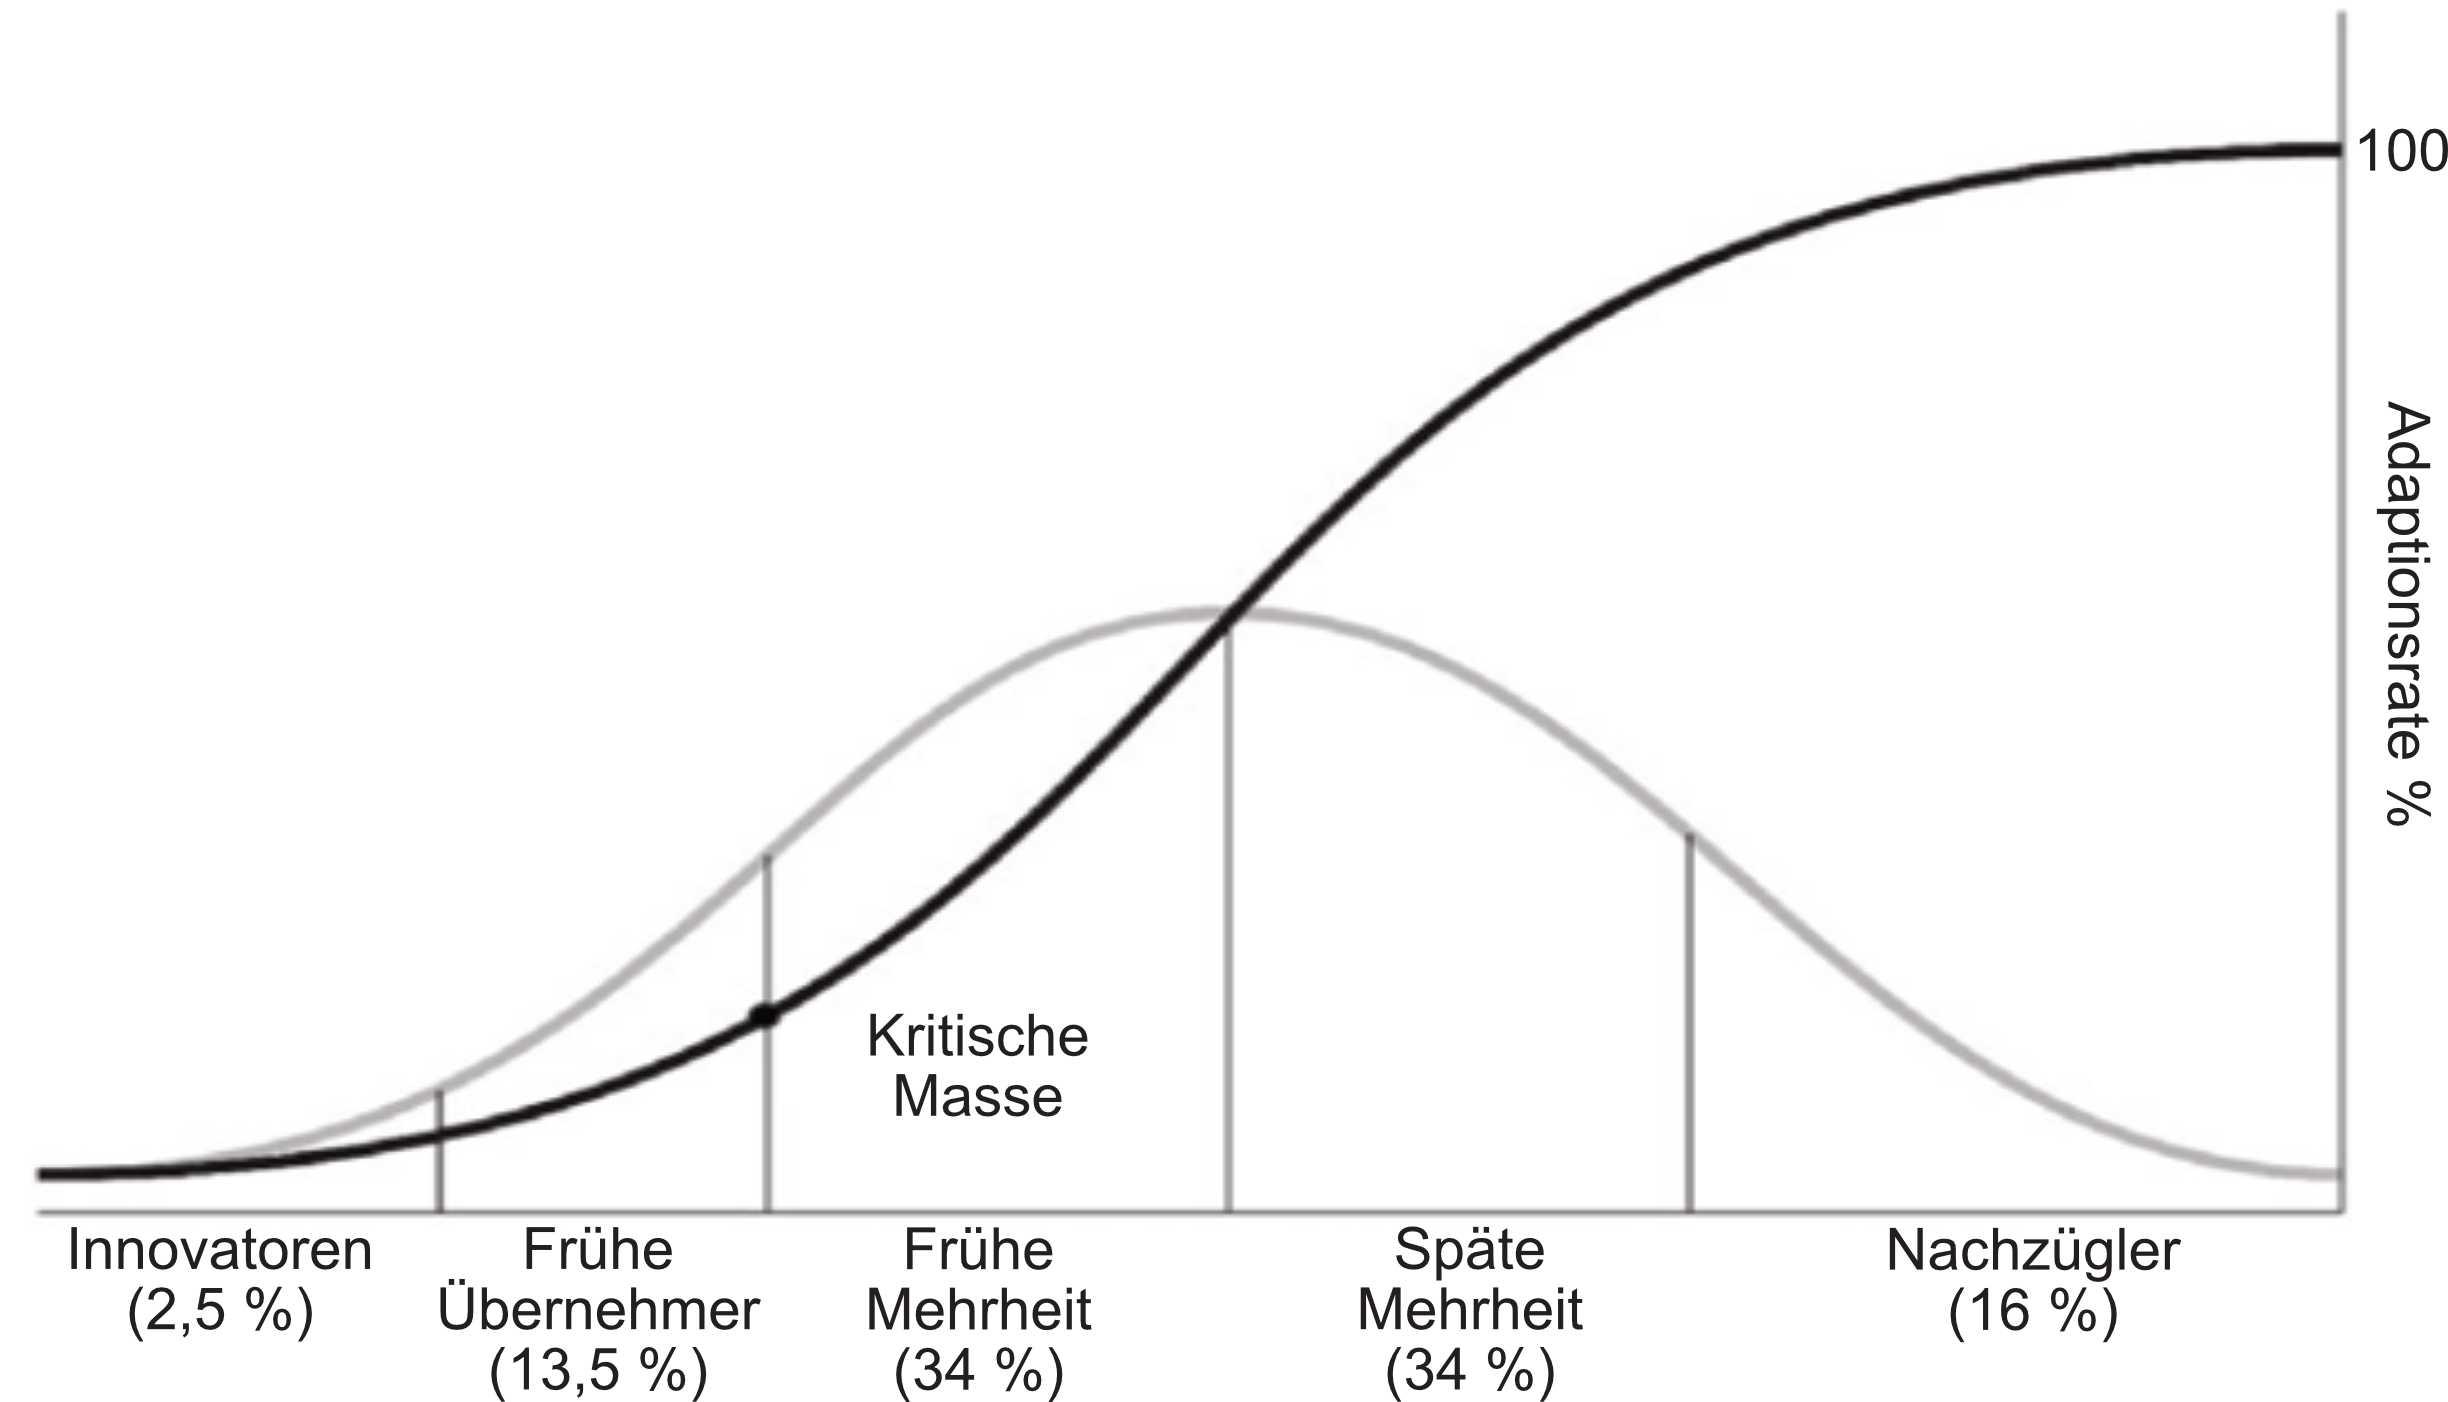
\includegraphics[width=0.75\linewidth]{img/ID_Bild.png}
  \caption{Adaptionskurve / Grafische Darstellung der ID \cite{potthoff_diffusion_2016}}
  \label{fig:id}
\end{figure}

%-----------------------------------------------------
%------------------ Modelldesign ---------------------
%-----------------------------------------------------

\section{Modelldesign}\label{Modelldesign}
Im Folgenden wird genauer auf das in NetLogo implementierte ABM eingegangen, das den Simulationsexperimenten zugrunde liegt. Dabei handelt es sich um kognitive Agenten, die miteinander interagieren und sich so gegenseitig beeinflussen. 

Zur Beantwortung der Forschungsfrage werden verschiedene Annahmen und Abgrenzungen getroffen, um den Kern der Arbeit angemessen zu beleuchten und eine sinnvolle Abstraktion der realen Welt zu schaffen. 
Diese Annahmen und Abgrenzungen sind notwendig, um die Komplexität des Modells zu reduzieren und fundierte Ergebnisse zu erzielen. 
Diese erlauben es, die Dynamiken der Informationsausbreitung in sozialen Netzwerken auf eine Weise zu untersuchen, die sowohl theoretisch fundiert als auch praxisrelevant ist.
Demzufolge wird darauf verzichtet, Greenfluencer und Nutzende verschiedenen Alters, Geschlechts, Kultur und Bildungsstands sowie äußere Einflüsse auf das Modell, wie Naturkatastrophen oder politische Entscheidungen, abzubilden. 
Sämtliche private Kommunikation zwischen den Nutzenden wird im Modell nicht berücksichtigt und somit ein Fokus auf die öffentliche Kommunikation auf Post- bzw. Tweet-Ebene gelegt. 
In der gesamten Modellierung und allen Experimenten wird von einer epidemischen Informationsausbreitung ausgegangen \cite{abdullah_epidemic_2011}. 

\subsection{Netzwerkaufbau}

Das Netzwerkmodell ist inspiriert von Kaufmann et al. (2009) und basiert auf einer modifizierten Version des Small-World-Modells von Watts und Strogatz (1998), das um Elementen aus dem Preferential Attachment erweitert wurde. Ausgangspunkt für die Netzwerkimplementierung ist das Modell von Uri Wilensky, das an die spezifischen Anforderungen dieser Forschung angepasst wurde \cite{wilensky_small_2015}. 
%So stellt es nun ein dynamisches Netzwerk dar, das sowohl die Small-World-Eigenschaften als auch die ungleiche Verteilung von Verbindungen, wie sie im preferential attachment zu finden ist, kombiniert.
Im klassischen Small-World-Modell von Watts und Strogatz (1998) besteht die Anordnung von N Agenten in einem Ring, wobei jeder Agent zu seinen k direkten Nachbarn verbunden ist. Eine bestimmte Anzahl dieser ursprünglichen Verbindungen bleibt bestehen, während andere, gemäß einer Wahrscheinlichkeit p, mit einem zufälligen Agenten neu verdrahtet werden. %Der Parameter p steuert den Grad der Zufälligkeit im Netzwerk: Bei p=0 bleibt das Netzwerk vollständig geordnet, und bei p=1 wird das Netzwerk hochgradig zufällig. Für die Struktur des Netzwerks gilt dabei die Bedingung n $>$ k $>$ ln(n) $>$ 1. \cite{watts_collective_1998} 
%Für das vorliegende Modell sind n = 1000 und p = 0,9 festgelegt worden, mit der daraus resultierenden durchschnittlichen Anzahl an Verbindungen zu anderen Agenten von k = 7. Des Weiteren wurden gerichtete Verbindungen genutzt, um unter dem Agenten folgenden und denen vom Agenten gefolgten zu unterscheiden. 

Zusätzlich werden Elemente des Preferential Attachment's integriert. Dieses Konzept, ursprünglich von Barabási und Albert (1999) eingeführt, beschreibt Netzwerke, in denen wenige Knoten sehr viele Verbindungen aufweisen, während die Mehrheit der Knoten nur über wenige Verbindungen verfügt. Dadurch entstehen sog. „Hubs“, also stark vernetzte Knoten, die das Zentrum des Netzwerks bilden und die Greenfluencer repräsentieren \cite{barabasi_emergence_1999}.
Jedoch werden die Verbindungen, die neu zu verdrahten sind, unter den Greenfluencern aufgeteilt und nicht nach den, wie in der Theorie beschriebenen, Wahrscheinlichkeiten.
Dies ermöglicht eine gezielte Steuerung der Netzwerkdynamik, bei der die zentralen Knoten nicht zufällig entstehen, sondern bewusst als Greenfluencer definiert werden.

%Generell werden die Knoten zunächst mit ihren direkten Nachbarn verbunden, was der klassischen Small-World-Topologie entspricht und erst danach entsprechend dem Prinzip der Neuverdrahtung in Hinblick auf das Preferential Attachment modifiziert.


\subsection{Modell Setup}
Zu Beginn der Simulation werden die Agenten erstellt und 2,5\% dieser zufällig ausgewählt und zu Greenfluencern ernannt, was der Anzahl an Innovatoren in der Theorie der ID gleicht \cite{potthoff_diffusion_2016}. 
Anschließend wird das Netzwerk wie zuvor beschrieben aufgebaut. 
Im nächsten Schritt werden alle Agenten initialisiert, wobei die agentenspezifischen Variablen der Tabelle \ref{tab:turtle_vars} zu entnehmen sind. Diese sind gleichzeitig die Aspekte, aus denen sich die Intention des Agenten in diesem Modell zusammensetzt. Bei der initialen Haltung werden die dazugehörigen Werte entsprechend der ID bestimmt, indem die Agenten nach den bekannten Gruppenverhältnissen eingeteilt werden und absteigend mit dem Zeitpunkt der Adaption Werte für die Variablen, aus denen sich die Haltung zusammensetzt, erhalten (siehe Tabelle \ref{tab:turtle_vars}). So repräsentieren beispielsweise 13,5\% der Agenten die Frühe Mehrheit und erhalten für alle Variablen, aus denen sich die Haltung zusammensetzt, den Wert 0,8. Greenfluencer stellen unterdessen die Innovatoren dar und werden mit 1 initialisiert. % Zusätzlich zur initialen Haltung werden auch die übrigen Werte der Influencer mit 1 initialisiert.
In der Simulation operieren die Werte der Agenten (siehe Tabelle \ref{tab:turtle_vars}) grundsätzlich im Bereich $\{0, \ldots, 1\}$, wobei es möglich ist, dass diese Werte durch Interaktionen oder externe Einflüsse während der Simulation den definierten Wertebereich verlassen. 

\begin{table}[H]
\begin{tabular}{|l|l|l|}
\hline
\textbf{Variable} & \textbf{Belegung}  & \textbf{Bemerkungen}    \\ \hline
influencer?  & \{true, 0\}   & \begin{tabular}[c]{@{}l@{}}true, falls Agent Greenfluencer ist,\\ 0 andernfalls\end{tabular}  \\ \hline credibility & Zufallswert & Glaubwürdigkeit des Agenten  \\ \hline\textbf{attitude} & initial-attitude  &  \\ \hline
initial-attitude  & {[}0.2, 0.4, 0.6, 0.8, 1{]}  & basiert auf Gruppeneinteilung  \\ \hline comfort   & initial-attitude       & \begin{tabular}[c]{@{}l@{}}Bequemlichkeit des Agenten,\\ bleibt konstant\end{tabular}               \\ \hline env-awareness   & initial-attitude    & \begin{tabular}[c]{@{}l@{}}Umweltbewusstsein des \\ Agenten, ändert sich \\ basierend auf Interaktion\end{tabular} \\ \hline  \textbf{social-norm}   & initial-norm    &  \\ \hline
initial-norm     & Zufallswert   & \begin{tabular}[c]{@{}l@{}}noch keine Interaktion mit \\ dem sozialen Umfeld,\\ daher zufällig bestimmt\end{tabular} \\ \hline
\textbf{\begin{tabular}[c]{@{}l@{}}perceived-behavioral-\\ control\end{tabular}} & (condition + self-efficacy)/2 & \begin{tabular}[c]{@{}l@{}}Mittel der Rahmen- \\ bedingungen und \\ Selbstwirksamkeit\end{tabular}  \\ \hline self-efficacy    & Zufallswert          & Selbstwirksamkeit des Agenten  \\ \hline conditions  & Zufallswert          & \begin{tabular}[c]{@{}l@{}}Rahmenbedingungen des \\ Agenten (wie verfügbares \\ Geld und Zeit)\end{tabular}     \\ \hline \textbf{intention} & siehe Gleichung \ref{eq:intention}& Handlungsabsicht des Agenten  \\ \hline

\end{tabular}
\caption{Initiale Werte der Agenten}
  \label{tab:turtle_vars}
\end{table}

\subsection{Simulationsablauf}
Die Simulation schreitet mit jeder Zeiteinheit (Tick), die hier einen Tag repräsentiert, einen Schritt voran. In jedem Simulationsschritt werden Posts von Greenfluencern generiert, im Netzwerk verbreitet und Interaktionen der Agenten mit diesen Posts durchgeführt. Ziel ist es, die Veränderungen der Intentionen der Agenten hinsichtlich der Adaption des Bewusstseins für Natur- und Umweltschutz im Zeitverlauf zu erfassen. Um die Darstellung der Posts sowie die Erfassung aller relevanten Interaktionsdaten zu ermöglichen, wurde ein Post-Objekt implementiert. Dieses Objekt erlaubt es zusätzlich, Verbindungen zwischen den Agenten und den Posts herzustellen, sobald ein Agent einen Post sieht.

Im ersten Schritt werden alle Agenten, die eine direkte Verbindung zu einem Greenfluencer haben, mit dem Post verknüpft. Sobald diese Agenten mit dem Post interagiert haben, wird der Post mit einer bestimmten Wahrscheinlichkeit an deren direkte Nachbarn weitergeleitet, was den Verbreitungsprozess im Netzwerk simuliert. Diese Diffusion der Posts dauert jeweils einen Tick an, sodass bei jedem neuen Tick die zuvor generierten Posts entfernt und durch neue Posts ersetzt werden. Die Anzahl der Posts, die ein Greenfluencer pro Tick erstellt, hängt dabei von einer Kategorie ab, die ihm zu Beginn jedes neuen Ticks zugewiesen wird und sich an der Tabelle \ref{tab:influencer_types} orientieren. 

\subsubsection{Postinteraktion} 
Die Interaktion mit dem Post ist der Zeitpunkt der Simulation, in der sich die Werte des Agenten, wie Haltung oder PBC und damit auch die Intention, ändern können. Die Berechnung der Haltung, sozialen Norm und PCB gleicht mehrheitlich der Methodik von Schwarz und Ernst (2009), wobei die Formel für die soziale Norm für diesen Use Case angepasst wurde. So wird die soziale Norm des Agenten bei jeder Interaktion an die Norm des Gegenübers angepasst, statt die Norm gleich dem Durchschnitt der Intentionen der Nachbarschaft zu setzen.
Die Interaktion beschränkt sich dabei auf das reine Sehen, Liken, Kommentieren, Lesen dieser Kommentare sowie Teilen des Posts. Beim Teilen erstellt der Agent dabei ein neues Post-Objekt, das wie gehabt im Netzwerk verteilt und verarbeitet wird. Während der Interaktionen sowie beim Sehen eines Posts wird die Haltung und das PCB beeinflusst. Posts, deren Intention ähnlich der des Agenten sind, erhöhen diese Werte, während sie von Posts mit divergierenden Intentionen gesenkt werden. Dies entspricht der Rolle externer Informationen bei Schwarz und Ernst (2009). Die soziale Norm wird dahingegen bei der Betrachtung eines neuen Posts und beim Lesen von Kommentaren beeinflusst, da dies der einzige Zeitpunkt ist, zu dem der Agent in Berührung mit der Meinung des sozialen Umfelds kommt. 


Nach der Interaktion wird die Intention neu berechnet. Wie die Arbeit von Schwarz und Ernst (2009) sowie die Forschung von Liao (2024) zeigen, spielt die soziale Norm nur eine geringe Rolle bei der Bestimmung der Intention, weshalb sie auch hier geringer gewichtet wird, als die zwei übrigen Aspekte Haltung und PBC \cite{schwarz_agent-based_2009,liao_exploring_2024}. Die Gewichte von der Haltung (w\textsubscript{a}) und PCB (w\textsubscript{pbc}) entsprechen beide 0,5 und das Gewicht der sozialen Norm (w\textsubscript{sn}) wird für alle Agenten auf 0,3 festgelegt, ausgenommen sind hier jedoch die Greenfluencer in ihrer Rolle als Meinungsführer. Bei ihnen beträgt das Gewicht 0. Die einzelnen Berechnungen werden wie folgt durchgeführt:

\begin{equation}
  \text{intention} = (\text{w}_{\text{a}} \cdot \text{attitude} + \text{w}_{\text{pbc}} \cdot \text{pbc}) \cdot (1 - \text{w}_{\text{sn}}) 
  + (\text{w}_{\text{sn}} \cdot \text{social-norm})
  \label{eq:intention}
\end{equation}

\begin{equation}
  \text{attitude} = 0.5 \cdot (\text{env-awareness} + \text{interaction-impact}) 
  + 0.5 \cdot \text{comfort}
  \label{eq:attitude}
\end{equation}

\begin{equation}
  \text{pbc} = 0.5 \cdot (\text{conditions} + \text{interaction-impact} + \text{self-efficacy})
  \label{eq:pbc}
\end{equation}

\begin{equation}
  \text{social-norm} = \text{social-norm} + \text{sender-impact} \cdot (\text{sender-intent} - \text{social-norm})
  \label{eq:social-norm}
\end{equation}

Der \textit{sender-impact} bei dem originalen Post des Greenfluencers ist mit 0,1 doppelt so hoch wie bei einem Post von einem Agenten, der kein Greenfluencer ist. Da eigene Posts von Agenten nicht berücksichtigt werden, handelt es sich dabei um einen Post, der vom Greenfluencer erstellt und anschließend von einem der Agenten geteilt wurde. Gleiches gilt für das Lesen der Kommentare, auch hier beträgt der \textit{sender-impact} 0,05. Ausgenommen von dieser Beeinflussung der sozialen Norm sind jedoch die Greenfluencer, da sie gegenüber Einflüssen aus ihrem sozialen Umfeld immun sind/ als immun gelten \cite{schwarz_agent-based_2009,kaufmann_simulating_2009}.

\subsubsection{Netzwerkanpassungen}
Im Anschluss zur Adjustierung der Intention nach jeder Postinteraktion werden Anpassungen am Netzwerk durchgeführt, die sich auf das Entfernen von bestehenden und Hinzufügen von neuen Links beschränken. Dabei gilt: Wenn der Agent dem Greenfluencer nicht bereits folgt und die Intentionen ähnlich sind, wird mit einer bestimmten Wahrscheinlichkeit ein neuer Link vom Agenten zum Greenfluencer erstellt, wodurch der Agent dem Greenfluencer nun folgt. Falls der Agent dem Greenfluencer folgt, aber die Absichten nicht (mehr) ähnlich sind, wird die bestehende Verbindung mit einer festgelegten Wahrscheinlichkeit entfernt, der Agent folgt dem Greenfluencer somit nicht mehr.

\subsection{Verifikation, Kalibrierung und Validierung}
Der Modellierungsprozess wurde als iterativer Entwicklungsprozess durchgeführt, bei dem kontinuierlich neue Funktionalitäten hinzugefügt, direkt evaluiert und getestet wurden, um die Entstehung von Fehlern zu minimieren. Diese Vorgehensweise stellt sicher, dass jeder Schritt der Modellentwicklung durch eine fortlaufende Verifikation begleitet wird. 
Die weiteren Schritte wurden nach der Methodik von Klügl (2008) durchgeführt. Angefangen wird mit der Kalibrierung des Modells, deren Ziel es ist, die Modellparameter so einzustellen, dass die Abweichung zwischen dem Modelloutput und den realen Daten minimiert wird und so ein Optimierungsproblem darstellt. Dies wird erreicht, indem die Modellparameter so justiert werden, dass das Modell sowohl strukturell korrekt ist als auch gültige Ergebnisse liefert, die größtmöglich mit der Realität übereinstimmen \cite{klugl_validation_2008}. In dieser Arbeit wurde die Kalibrierung mit dem NetLogo ergänzenden Tool „Behaviorsearch“ durchgeführt, wobei insbesondere die folgenden Parameter untersucht wurden:

\begin{enumerate}
  \item Der Schwellenwert, ab wann ein Agent als Adaptierer gilt.
  \item Die Wahrscheinlichkeiten, mit denen ein Agent einem Greenfluencer folgt oder entfolgt, wodurch die Netzwerkanpassungen stattfinden. 
  \item Die Wahrscheinlichkeiten, mit denen ein Agent ein Post liked, kommentiert oder teilt. 
\end{enumerate}

Im Rahmen der sog. Face Validation wurde das Modell und seine Interaktionsmechanismen einer detaillierten Überprüfung unterzogen, um sicherzu- stellen, dass die beobachteten Effekte plausibel und das Modellverhalten erwartungsgemäß sind. Die Face Validation ist ein qualitativer Ansatz, der darauf abzielt, die Korrektheit des Modells durch visuelle Bewertung zu bestätigen \cite{klugl_validation_2008}. In der visuellen Bewertung werden zunächst die Animationen des Netzwerkes gründlich analysiert, wobei besonders darauf geachtet wurde, dass keine auffälligen oder unerwarteten Verhaltensweisen auftreten und die Netzwerkstruktur als plausibel eingestuft werden kann.
Des Weiteren wurde das gesamte Verhalten des Modells im Rahmen der Ergebnisbewertung beobachtet, wobei sich zeigte, dass die erzeugten Graphen korrekte Relationen abbilden. Beispielsweise fällt die Zahl der mäßig interessierten Agenten schneller als die der Nicht-Adaptierer, was darauf hinweist, dass die mäßig Interessierten schneller zu Adaptierern werden, während die Nicht-Adaptierer länger benötigen, um ihre Haltung zu ändern. Schließlich wurden bei der immersiven Bewertung einzelne Agenten im Detail beobachtet, um deren interne Zustände, Handlungen und Reaktionen auf Posts sowie die Interaktionen mit Greenfluencern und Nicht-Greenfluencern nachvollziehen zu können. Diese vertieften Beobachtungen ermöglichen ein besseres Verständnis für das Verhalten der Agenten und tragen zur Bestätigung der Korrektheit und Plausibilität der Mikrointeraktionen im Modell bei.
 
Zusätzlich wurde eine Suche nach Ausreißern durchgeführt. Dabei wurden die Werte für die Intention, Haltung, PBC und sozialen Norm der Agenten überprüft. Es treten keine unplausiblen Werte auf, die als Ausreißer interpretiert werden können. Mehrere Simulationsläufe bestätigen diese Ergebnisse, da alle Läufe ähnliche Resultate hervorbringen und keine untypischen Simulationsergebnisse erkennbar sind.
Insgesamt kann auf Basis dieser Validierungen sowie der erfolgreichen Kalibrierung mit verschiedenen Realdaten auf die Validität des Modells geschlossen werden. Die Annahmen und die Struktur des Modells gelten als verifiziert und die durchgeführten Tests bestätigen die Zuverlässigkeit des Modells in Bezug auf seine Fähigkeit, realistische und plausibel erscheinende Ergebnisse zu liefern.


%-----------------------------------------------------
%------------------ Experimente ----------------------
%-----------------------------------------------------
\section{Simulationsexperimente}\label{Simulationsexperimente}
Die nachfolgenden Simulationsexperimente zielen darauf ab, die Auswirkungen verschiedener Parameter auf die ID aufzuzeigen. Dabei fokussieren die Experimente die, durch das Netzwerk und den Greenfluencer beeinflussbare, Parameter. 
Es wird explizit darauf verzichtet, verschiedene Änderungen in der TPB durchzuführen, da diese Parameter als durch den Nutzenden gegeben angesehen werden. 
Die nachfolgenden Experimente wurden für je 400 Ticks mit 10 Durchläufen durchgeführt, um kleinere Modellvarianzen zu berücksichtigen. 
Vorab wurde die Modellvarianz untersucht und festgestellt, dass die eingesetzten Random Seeds keine relevanten Auswirkungen auf das Modellverhalten haben. 

\subsection{Erhöhung der Anzahl der Agenten}
\begin{itemize}
  \item \textbf{Hypothese}: Mit der Erhöhung der Gesamtzahl der Agenten im Netzwerk, begleitet von einer proportionalen Zunahme der Greenfluencer, wird die ID verlangsamt. Trotz der Zunahme der Greenfluencer wird die größere Netzwerkkapazität zu einer erhöhten Diversität und Heterogenität der einzelnen Agenten führen. Dies verlängert die notwendige Zeit zur vollständigen ID, da die Innovationsinhalte über eine größere Anzahl von Agenten verteilt werden müssen.
  \item \textbf{Fallbeispiel}: Das soziale Netzwerk X gewinnt an Nutzenden und dadurch auch an Influencern.
  \item \textbf{Design}: Simulation mit variierender Anzahl von Agenten (Anzahl: 1000 – 2000, Standard: 1000), bei proportionaler Erhöhung der Greenfluencer.
  \item \textbf{Messgrößen}: Geschwindigkeit der vollständigen ID.
  \item \textbf{Ergebnis}: Das Ergebnis des ersten Experiments legt dar, dass die Anzahl der Agenten keinen Einfluss auf die Geschwindigkeit der ID hat (siehe \ref{fig:e1u2u3}).
  \item \textbf{Interpretation}: Das Experiment widerspricht der ursprünglichen Hypothese, dass eine größere Anzahl von Agenten, begleitet von einer proportionalen Zunahme der Greenfluencer, die Diffusion verlangsamt. Stattdessen deutet das Ergebnis darauf hin, dass die ID in diesem Netzwerk robust gegenüber Veränderungen  der Agentenanzahl ist. Das Ergebnis könnte durch die Eigenschaften von Small-World-Netzwerken erklärt werden. Bei denen durch die hohe Clustering-Rate, Innovationen effizient verbreitet werden können, obwohl das Netzwerk wächst. Dadurch kann die zusätzliche Anzahl an Agenten möglicherweise besser kompensiert werden. Im Kontext des Modells ist das Ergebnis nachvollziehbar und zeigt die Robustheit und Effizienz von Small-World-Netzwerken.
\end{itemize}

\subsection{Erhöhung der Postanzahl pro Greenfluencer}
\begin{itemize}
  \item \textbf{Hypothese}: Eine Erhöhung der Anzahl der von Greenfluencern generierten Posts (Innovationsinhalte) wird die Geschwindigkeit der ID steigern, da die erhöhte Präsenz und Sichtbarkeit der Innovation zu einer höheren Wahrscheinlichkeit führt, dass Agenten die Innovation wahrnehmen.
  \item \textbf{Fallbeispiel}: Greenfluencer erhöhen Ihre Postanzahl und werden aktiver. 
  \item \textbf{Design}: Simulation mit erhöhter Postanzahl der Influencer-Gruppen (Faktor: 1, 2, 3 Standard: 1).
  \item \textbf{Messgrößen}: Geschwindigkeit der vollständigen ID.
  \item \textbf{Ergebnis}: Die Erhöhung der Anzahl von Posts pro Greenfluencer führt in diesem Experiment zu einer anfänglich schnelleren Ausbreitung der Innovation. Je weiter die Simulation voranschreitet, desto geringer werden die Unterschiede, bis diese zu Ende des Experiments eine geringe Abweichung von unter 1 \% darstellen (siehe \ref{fig:e1u2u3}). 
  \item \textbf{Interpretation}: Das Ergebnis bestätigt die Hypothese und zeigt auf, dass die anfänglich großen Unterschiede der Diffusionsgeschwindigkeit mit fortschreitendem Verlauf des Experiments zunehmend geringer werden, was darauf hindeutet, dass die anfänglichen Vorteile einer höheren Postfrequenz nicht mehr den gleichen Einfluss auf die Diffusionsgeschwindigkeit haben. Eine mögliche Erklärung dafür ist, dass für die Innovation anfällige Agenten diese bereits frühzeitig übernehmen und allmählich der zusätzliche Einfluss vermehrter Posts an Effektivität verliert.
\end{itemize}

\subsection{Erhöhung der Engagement-Rate}
\begin{itemize}
  \item \textbf{Hypothese}: Die Erhöhung der Engagement-Rate (Interaktionshäufigkeit mit Posts) wird die ID beschleunigen, da Agenten, durch das stärker Interagieren mit den Innovationsinhalten  (durch Liken, Kommentieren oder Teilen), die Verbreitung dieser im Netzwerk fördern und so andere Nutzer besser von der Innovation erreicht werden können. 
  \item \textbf{Fallbeispiel}: Durch das Einbinden von multimedialen Inhalten oder Hashtags kann die Engagement-Rate erhöht werden \cite{wadhwa_maximizing_2017}.
  \item \textbf{Design}: Modifikation der Lesewahrscheinlichkeit (0,5; 0,6; 0,7; 0,8; 0,9; 1) und dadurch der Anzahl der Likes, Kommentare und geteilten Beiträge. 
  \item \textbf{Messgrößen}: Geschwindigkeit der vollständigen ID.
  \item \textbf{Ergebnis}: Durch das Erhöhen der Engagement-Rate bzw. der Lesewahrscheinlichkeit konnte die ID beschleunigt werden (siehe \ref{fig:e1u2u3}).
  \item \textbf{Interpretation}: Die Untersuchung bestätigt die Hypothese und zeigt auf, dass durch eine erhöhte Interaktionswahrscheinlichkeit, Agenten aktiver mit den Inhalten interagieren und so nicht nur die Reichweite der Innovation erhöht wird, sondern auch die einzelnen Elemente der TPB verstärkt werden, was die soziale Akzeptanz der Innovation fördert. Zusammengefasst deutet dies darauf hin, dass die Förderung der Engagement-Rate durch gezielte Maßnahmen, wie das Einbinden von multimedialen Inhalten oder die Nutzung von Hashtags, ein wirksames Mittel ist, um die ID zu beschleunigen. Die Interaktion der Agenten spielt eine zentrale Rolle dabei, wie schnell und weitreichend eine Innovation angenommen wird.
\end{itemize}
\begin{figure}
  \centering
  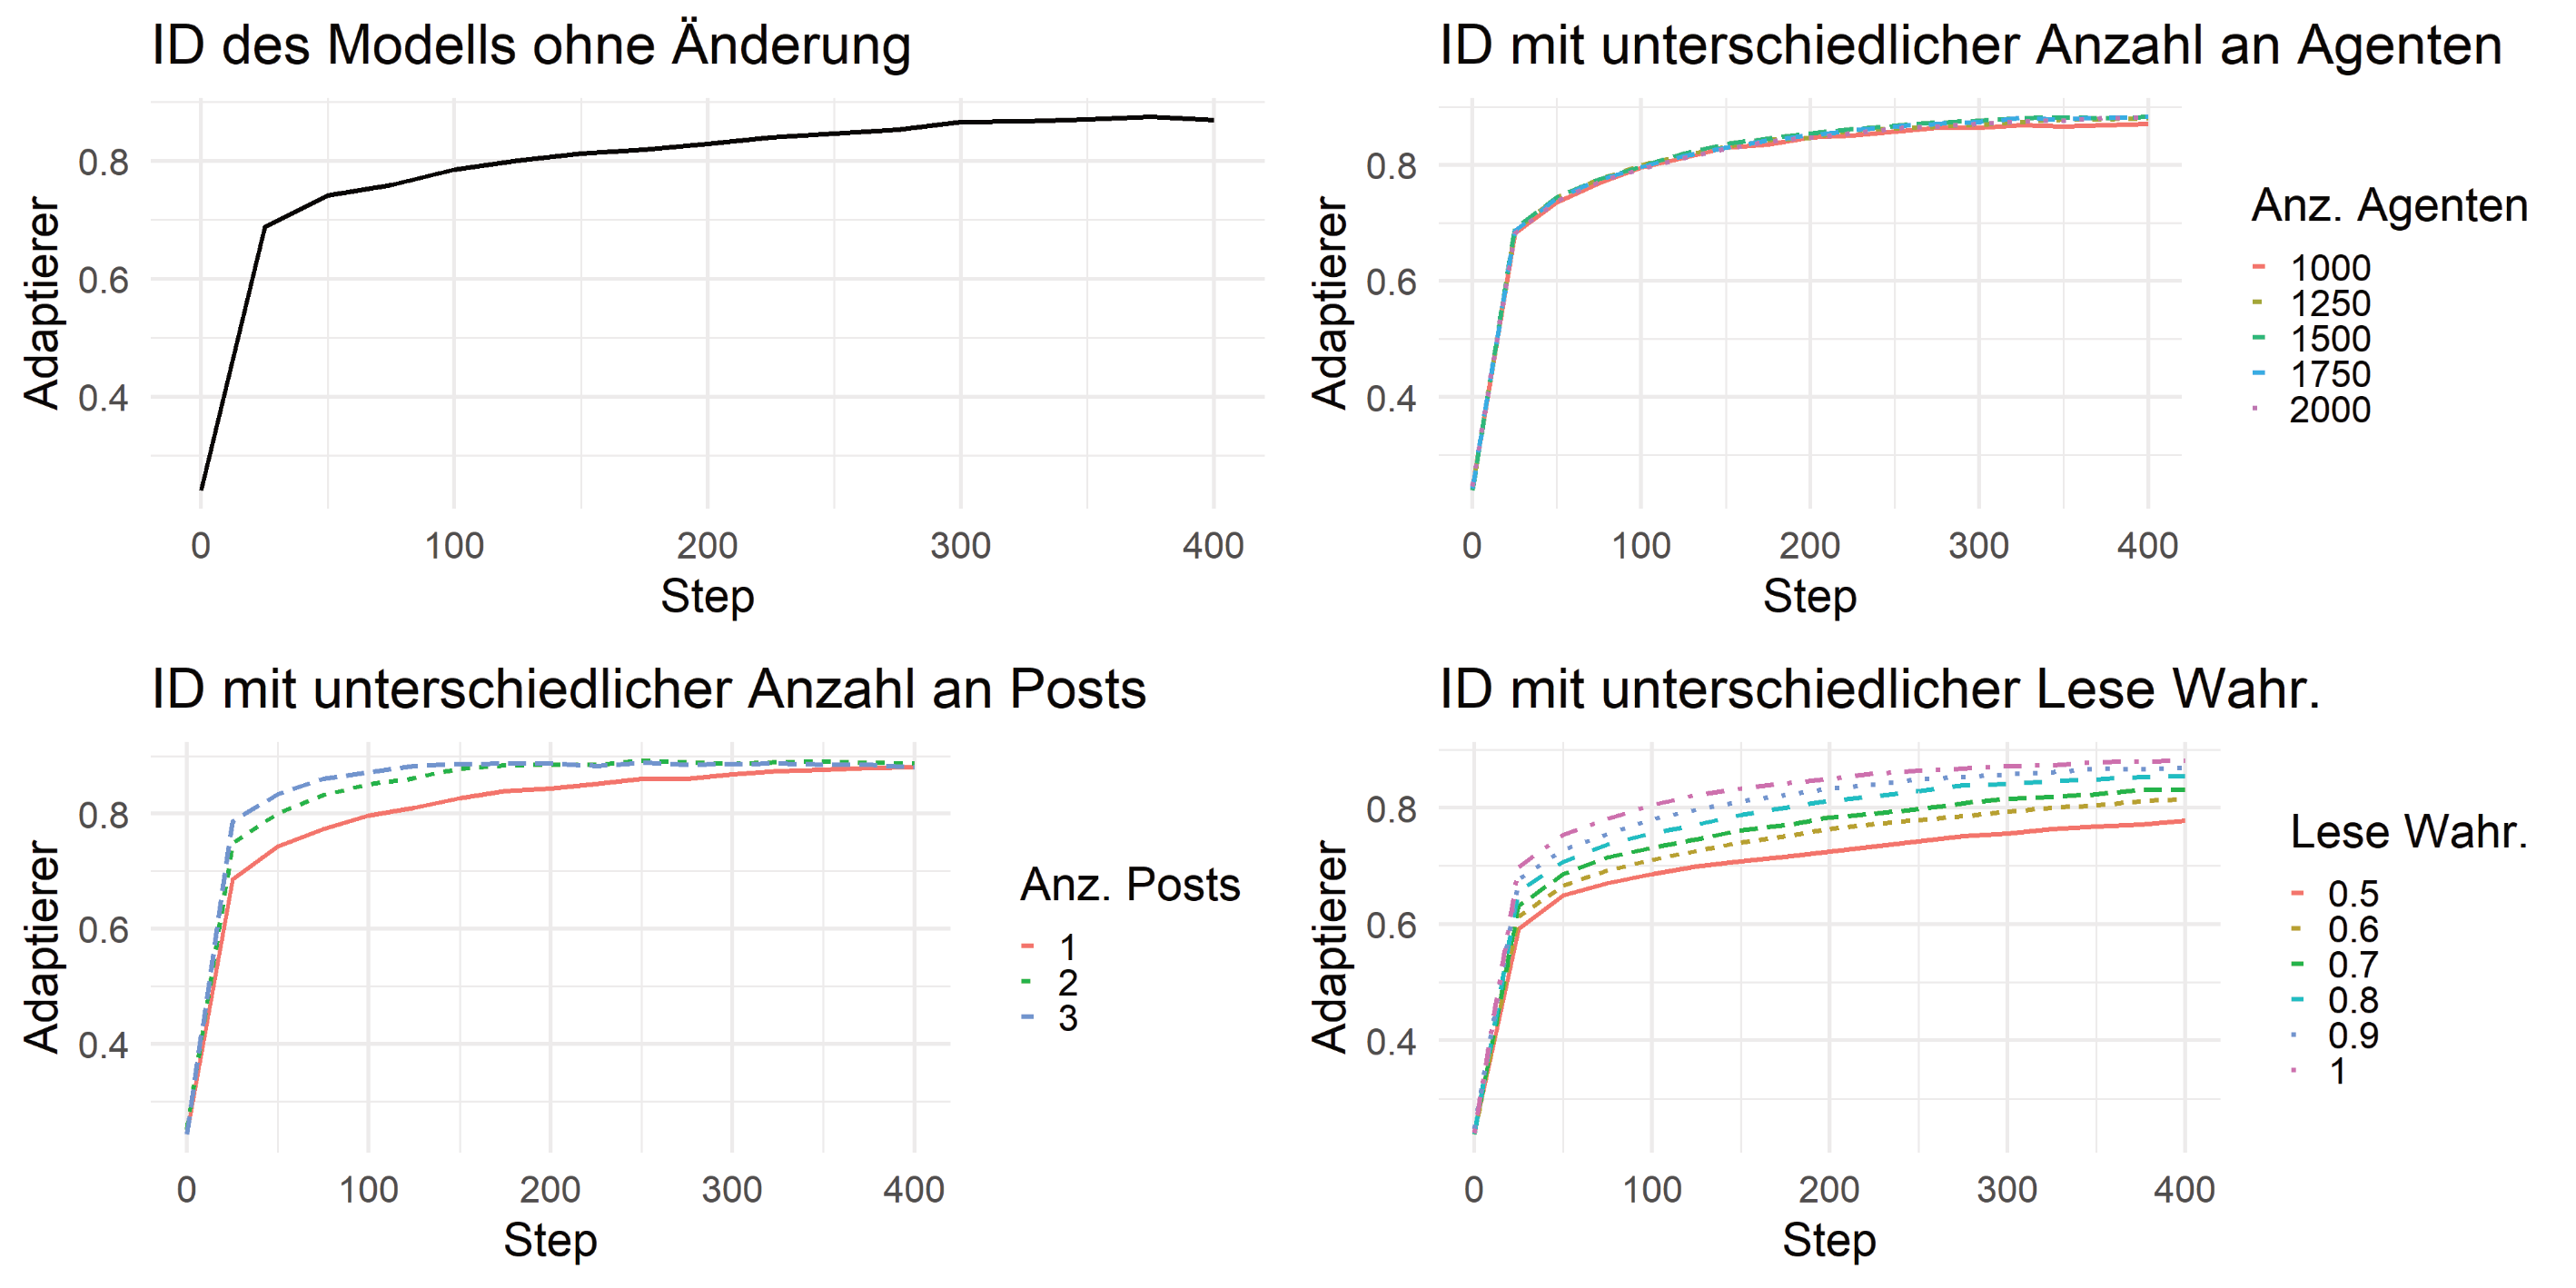
\includegraphics[width=1\linewidth]{img/e1u2u3.png}
  \caption{Ergebnis der ID und Experiment 1, 2 und 3}
  \label{fig:e1u2u3}
\end{figure}


\section{Fazit und Ausblick}
Das vorangegangene Paper untersucht die Korrelation zwischen den psychologischen Modellen der ID und der TPB im sozialen Netzwerk X (ehemals Twitter). 
Dabei wird ein klarer Zusammenhang zwischen nachhaltigen Themen, die durch Greenfluencer vorangetrieben werden, und sozialen Medien hergestellt.
Dies geschieht, indem die, für soziale Medien und nachhaltige Themen, üblichen Strukturen, insb. durch die Anzahl der Follower und den Fokus auf Greenfluencer der Kategorien „Regular“ und „Micro“ (siehe \ref{tab:influencer_types}) nachgebildet werden. 
Zusätzlich werden bei der Haltung der Agenten Aspekte wie das bestehende Umweltbewusstsein oder die Bequemlichkeit des Agenten berücksichtigt. 
Die Forschung zeigt deutlich, dass sich die ID unter der Anwendung der TPB in sozialen Medien darstellen lässt. \\
\indent Ersichtlich ist dies insbesondere durch den Verlauf der Innovation (siehe Abb. \ref{fig:e1u2u3}) innerhalb des ABMs. Hier ist zu erkennen, dass die Adaptionsrate erst rasant bis zu 70 \% steigt und ab dort verlangsamt wächst. Für die ID bedeutet das rasante Wachstum, dass hier die Frühe Mehrheit sowie ein Teil der Späten Mehrheit erreicht wurde und die Innovation adaptiert hat. Ausgenommen sind hier die Frühen Übernehmer, diese haben die Innovation bereits vor Beginn der Untersuchung adaptiert, was die Realität abbildet \cite{ifd_allensbach_naturschutz_2023}. Die Adaptionskurve bestätigt dieses Verhalten, da hier der Hochpunkt genau zwischen den beiden Gruppen liegt (siehe Abb. \ref{fig:id}), was eine schnelle ID bedeutet, dann jedoch rasant abflacht, was eine verlangsamte ID zur Folge hat. Verhältnismäßig ist die Geschwindigkeit, in der der Rest der Späten Mehrheit erreicht wird, jedoch geringer, als in der Abbildung \ref{fig:id} der Adaptionskurve ersichtlich, die Anzahl an Adaptieren ist hingegen korrekt. Anschließend wächst die Adaptionsrate jedoch nur bis ca. 87 \% und stagniert von dort an. So adaptieren, anders als in der klassischen ID, ein Großteil der Nachzügler die Innovation nicht. Da der soziale Druck, genauer gesagt die soziale Norm, in der Berechnung der Intention als weniger relevant erachtet wird \cite{schwarz_agent-based_2009,liao_exploring_2024}, genau dieser jedoch für die Nachzügler ausschlaggebend für die Adaption ist, gibt es einen bestimmten Teil an Agenten, der nicht adaptiert. Zusätzlich gibt es Agenten, die zwar Teil des Netzes sind, aber keine oder kaum ausgehende Verbindungen haben und entsprechend kaum oder gar nicht mit den Posts der Greenfluencer oder den Greenfluencern selbst in Kontakt treten. 
Dieses Ergebnis kann dahingegen auch darauf hindeuten, dass neben den in der TPB berücksichtigten Faktoren weitere Elemente eine Rolle spielen könnten, die das Verhalten der Agenten beeinflussen und die voll umfassende Adaption verhindern. 
Die durchgeführten Experimente stützen dabei die vorangegangene Forschung und zeigen die Wirkung unterschiedlicher Faktoren auf die ID. So zeigt die Erhöhung der Anzahl an Agenten keinen bedeutenden Einfluss, die Aktivität der Greenfluencer sowie die Gestaltung ihrer Beiträge zeigen andererseits einen Einfluss auf die ID. \\
\indent
Zusammenfassend zeigt diese Arbeit, dass die ID in sozialen Medien mittels der TPB modelliert werden kann. Besonders hervorzuheben ist dabei, dass der Modellaufbau und die Kalibrierung primär auf die Analyse der Interaktionen innerhalb des Netzwerks ausgerichtet wurden. Die Bestätigung der ID war hierbei nicht das primäre Ziel, sondern ergab sich als sekundärer Effekt des Nachbildens sozialer Netzwerke, was für die Unvoreingenommenheit des Modells sowie Robustheit der Ergebnisse spricht.

Wichtig zu beachten ist, dass das Modell ein hohes Abstraktionsniveau besitzt und nicht beachtete Aspekte wie Alter, Geschlecht, Kultur und Bildungsstand von Agenten sehr wohl Auswirkungen auf die ID in sozialen Medien haben können.
Insbesondere bei komplexen und kontroversen Themen oder Krisensituationen verbreiten sich Informationen nicht immer gleichmäßig, sondern werden oft durch den Algorithmus sozialer Medien aggressiver verteilt als andere Themen \cite{jiang_building_2021}. 
Ebenso stellt das Modell nur einen kleinen Auszug aus der Verbreitung von Innovationen dar und berücksichtigt keine äußeren Faktoren sowie private Kommunikationen bzw. Interaktionen und besitzt daher nur geringe Anwendbarkeit auf eine ganzheitliche ID in der Gesellschaft. 

Anwendung könnte diese Forschung zukünftig z. B. in Werbe- bzw. Nachhaltigkeitskampagnen finden, um Unterstützung bei der Entwicklung effektiver Strategien zur Förderung von Neuheiten und umweltfreundlichen Verhaltens- weisen in sozialen Medien zu bieten. 
Für die weitere Forschung wäre es zusätzlich interessant, wie sich Innovationen in sozialen Medien durchsetzen, wenn Influencer mit gegensätzlichen Meinungen involviert sind oder bewusst Falschinformationen verteilt werden. 
Die Forschung ist dabei nicht auf Nachhaltigkeitsthemen beschränkt, vielmehr lassen sich auch Themen wie technologische Innovationen, neue Zahlungsmethoden oder medizinische Fortschritte untersuchen. Im Allgemeinen umfasst dies alle Bereiche, in denen Meinungen, Lebensstile oder Produkte innerhalb eines Netzwerks verbreitet werden.
Hierbei wäre es interessant zu untersuchen, inwieweit gegensätzliche Positionen die Akzeptanz und Verbreitung von Innovationen beeinflussen oder diese sogar verhindern können und was für eine Rolle und Bedeutung falsche Informationen in diesem Zusammenhang spielen.
Ein weiteres vielversprechendes Forschungsthema wäre die Analyse der Auswirkungen des Social-Media-Algorithmus auf die ID, insbesondere wie Änderungen in der Postverteilung an themeninteressierte Nichtfollower, die Verbreitung und Akzeptanz von Innovationen beeinflussen. Diese Forschung könnte wichtige Erkenntnisse darüber liefern, wie soziale Netzwerke und ihre Algorithmen als Vermittler von Innovationen fungieren.


%
% ---- Bibliography ----
%
% BibTeX users should specify bibliography style 'splncs04'.
% References will then be sorted and formatted in the correct style.
%

%
%\begin{thebibliography}{8}
   \bibliographystyle{splncs04}
  \bibliography{src/references}
%\end{thebibliography}
\end{document}